% One time per channel: charge spreading and the track-angle bias of time-projection readouts.
% Review + unified model + MX17 chamber A as the test bed.  Draft 2026-11-09 (first full draft written by Claude at
% Dylan's request; every number comes from NUMBERS.md, generated by scripts/collect_numbers.py; figures from
% scripts/make_figures.py).  Target: a long NIM A / JINST article or an instrumentation review.  Author list undecided.
\documentclass[11pt,a4paper]{article}
\usepackage[margin=2.2cm]{geometry}
\usepackage[T1]{fontenc}
\usepackage{lmodern}
\usepackage{amsmath,amssymb}
\usepackage{graphicx}
\usepackage{booktabs}
\usepackage{array}
\usepackage{siunitx}
\usepackage{xcolor}
\usepackage[hidelinks]{hyperref}
\usepackage{cleveref}
\usepackage{microtype}
\sisetup{separate-uncertainty=true, range-phrase=--, range-units=single}
\graphicspath{{figures/}}

% drafting marks (remove for submission)
\newif\ifdraftnotes \draftnotestrue
\newcommand{\tbw}[1]{\ifdraftnotes{\color{red!70!black}[\textbf{tbw:} #1]}\fi}
\newcommand{\note}[1]{\ifdraftnotes{\color{blue!60!black}[\textit{note:} #1]}\fi}
\newcommand{\tand}{\tan\theta}
\newcommand{\um}{\si{\micro\metre}}

\title{One time per channel: how lateral charge spreading biases track angles in time-projection readouts, and what to do about it}
\author{D.~Neff$^{a,b}$ \tbw{author list to be decided with the MX17 collaboration}\\
\small $^a$Department of Physics and Astronomy, University of California, Los Angeles\\
\small $^b$CERN, Geneva}
\date{Draft of \today}

\begin{document}
\maketitle

\begin{abstract}
A micro time-projection chamber ($\mu$TPC) reconstructs a short track segment from the positions of its readout channels and one
drift time per channel. Since the first Micromegas and GEM implementations the reconstructed angle has been reported too large,
most strongly for tracks near normal incidence; the explanation in print is capacitive coupling between neighbouring strips, and
the remedies are edge-strip filters, a subtraction of a tuned fraction of the neighbour pulse, or an angle calibration. We review
this literature across detector families, from strip $\mu$TPCs to large pad TPCs, liquid-argon TPCs and directional recoil
detectors, and show that one mechanism covers all of it: a single time per channel is a functional of the charge from every
drift depth that reaches the channel, and any lateral spread of that charge (drift diffusion, the induction footprint, capacitive
coupling, resistive spreading) feeds the strips at the two ends of the column with charge of the wrong depth. For a straight
fit through $N$ channels the slope error is a strip-end term, $\tan\theta_{\rm rec}/\tan\theta - 1 \simeq C/N^2$, plus a small
interior term from the growth of the spread with depth; $C$ is set by the lateral spread in units of the pitch and by the time
estimator. We test this on a 28~mm resistive-strip Micromegas with a 0.78~mm pitch, 60~ns sampling and an external silicon
reference: on 50\,000 track projections the hit-time compression is $C = 7.0$ (X) and $11.7$ (Y) with no interior term
($|b|<0.02$), a forward model of the waveforms reproduces $C$ to 2\,\%, a geometry-only model gives $C = 2.3$, and the published
strip-$\mu$TPC points fall between the two. Depth-resolved stacking of the strip waveforms separates the same-time share at the mesh
(equivalent to a Gaussian of \SIrange{0.33}{0.37}{mm} on the view across the resistive strips, narrower along them) from a growth
with drift time that matches a transverse diffusion of $\approx\SI{350}{\micro\metre\per\sqrt{cm}}$, and shows a same-time second-neighbour share of
$2.4\,\%$ per side that no Gaussian footprint produces. A position-in-strip test, with its closure, bounds a pure nearest-neighbour
coupling well below the published \SIrange{15}{30}{\%}. The literature's remedies, scored on the same tracks against the reference,
remove at most two thirds of the bias and leave the angle resolution at \SIrange{1.5}{2}{} times that of a per-event forward fit of
the waveforms, which is unbiased to 1\,\%. We give the scaling needed to judge when a readout will see the effect and a recipe for
the measurements that separate its causes.
\end{abstract}

\tableofcontents

\section{Introduction}\label{sec:intro}

A time-projection readout turns a drift time into a coordinate. In a large TPC the drift coordinate is read along a track
many centimetres long and the local direction comes from many pad rows; in a micro-TPC ($\mu$TPC) the whole drift column is a
few millimetres to a few centimetres deep, each strip crossed by the track is given one drift time, and the inclination of the
segment is the slope of time against strip position~\cite{Alexopoulos2010,Bini2014}. The second form is attractive because it
recovers a good position for inclined tracks where the charge centroid degrades, and it is used in the ATLAS New Small Wheel
Micromegas~\cite{Iodice2015,Ntekas2016,Scholer2021}, in triple-GEM trackers~\cite{Alexeev2019,Farinelli2019,Flierl2018} and in
floating-strip Micromegas~\cite{Bortfeldt2014,Bortfeldt2015}.

Every one of these groups that compared the reconstructed inclination with the set angle of the chamber found the track too
steep, by a few degrees at \ang{10} shrinking to a fraction of a degree at \ang{40}~\cite{Bortfeldt2014,Iodice2015,Flierl2018,Ntekas2016}.
The published explanation is capacitive coupling: a strip at the edge of the cluster receives a copy of its neighbour's signal
at the neighbour's time, so the first and last strips carry the wrong depth~\cite{Bortfeldt2015,Iodice2015,Alexeev2019}. The
remedies are a cut on the charge ratio of the edge strips~\cite{Sessa2014,Rinnagel2019,Vanadia2015}, a shift of their assigned
position~\cite{Farinelli2019,Ntekas2016}, a subtraction of a fixed fraction of the neighbour pulse, sample by
sample~\cite{Loesel2017,Flierl2018,Herrmann2019}, or an angle-dependent calibration~\cite{Bortfeldt2014}. Two things are
missing from this record. No study has separated the coupling from the other processes that put charge of one depth on a
neighbouring strip, drift diffusion and the finite width of the induction footprint, and none has had a per-track external
reference for the angle: the comparison is always with the mounting angle of the chamber, through the peak or the mean of the
reconstructed distribution. Where the field's own simulations switch the coupling off they still find a bias, of \ang{0.2} to
\ang{4}~\cite{Ntekas2016} or \ang{7}~\cite{Scholer2021}, and leave it unexplained.

This paper argues that the question ``which process couples the strips'' is the wrong one for the angle. A single time per
channel, whatever its definition, is a functional of all the charge that reaches the channel, and the channels at the two ends of
a short column receive charge of the wrong depth from any lateral spread, by any mechanism. The bias is therefore a geometric
consequence of reading a short column one time per channel, its size is set by the lateral spread in units of the pitch and by the
number of channels in the column, and the mechanisms differ only in how they are to be modelled or removed. Pad TPCs and
liquid-argon TPCs have the same spread in units of the pitch but columns one or two orders of magnitude longer, and read a
charge-weighted time; directional and short-track detectors have the column but no reference that would reveal a few per cent
of slope. The strip $\mu$TPC is the one place where the effect is both large and measurable, and that is where it was found.

We test this account on a resistive-strip Micromegas with an unusually deep drift gap (\SI{28}{mm}), a fine pitch (\SI{0.78}{mm}),
sampled waveforms (\SI{60}{ns}) and a silicon telescope that gives the slope of every track independently of the chamber. The
detector, its calibration and its waveform reconstruction are described in two companion papers~\cite{paperI,paperII}; here it
serves as a test bed, with a forward model whose ingredients (footprint, diffusion, resistive spreading, electronics response)
can be switched on and off, and with 50\,000 track projections in two runs. \Cref{sec:formulation} sets out the formulation and
the scaling, \cref{sec:mechanisms} what the lateral spreads are and which observables separate them, \cref{sec:literature} what
each detector family has reported, \cref{sec:measurements} the measurements, \cref{sec:remedies} the remedies scored on the same
tracks, and \cref{sec:guidance} the consequences for the design and analysis of such readouts.

Terminology. We write $L$ for the drift length of the column, $p$ for the readout pitch, $v$ for the drift velocity, $\theta$
for the angle between the track and the drift direction, so that a track crosses $N = L\tan\theta/p$ strips, and $u$ for the
drift time of a charge from depth $z = v u$. ``Ratio'' means $\tan\theta_{\rm rec}/\tan\theta$ at fixed drift velocity, which is
also the factor by which the drift-time ladder is compressed; it is 1 for an unbiased reconstruction and larger than 1 when the
track reads too steep. ``Same-time'' sharing means charge appearing on a neighbour with the time structure of the strip's own
charge; ``delayed'' sharing means a later and longer signal, the signature of resistive spreading.

\section{The single-time estimator as a functional of the track segment}\label{sec:formulation}

\subsection{What a strip sees}

Consider a straight track through a drift gap of length $L$, inclined by $\theta$ to the drift direction, read by strips of
pitch $p$ (\cref{fig:schematic}a). Charge released at depth $z$ drifts for $u = z/v$ and arrives at the readout plane at
transverse position $x(z) = x_0 + z\tan\theta$, spread laterally by a distribution $f(x - x(z); z)$ of width $\sigma(z)$. The
current on strip $i$ is the sum over depths of the fraction of each depth's charge that lands within the strip, each folded
with the electronics response $T$:
\begin{equation}
  W_i(t) = \int_0^{L/v} du\; q(u)\, F_i(u)\, T(t - t_0 - u), \qquad
  F_i(u) = \int_{x_i - p/2}^{x_i + p/2} f(x - x(vu); vu)\, dx .
  \label{eq:waveform}
\end{equation}
With no lateral spread, $F_i$ is a box: strip $i$ collects exactly the depths $z_i \le z < z_i + \Delta z$ with
$\Delta z = p/\tan\theta$, over a time $\Delta t = p/(v\tan\theta)$. With a spread, strip $i$ also receives charge from depths
outside its box, from a range of order $\sigma(z)/\tan\theta$ on either side.

A hit-based readout keeps one time per strip, $t_i = \mathcal{E}[W_i]$, where the estimator $\mathcal{E}$ is a threshold crossing,
a leading-edge fraction of the peak, the time of the peak, a fitted rising edge, a time over threshold, or a charge-weighted
mean. The $\mu$TPC then fits a line $t_i = t_0' + x_i/w$ through the hits and reads the slope $w = dx/dt$ as $v\tan\theta_{\rm rec}$.
For an interior strip, with charge from both neighbouring depths on both sides, every estimator returns the time of some
representative depth within the strip's box, shifted by an amount that is the same for every interior strip when the spread is
the same at every depth: the interior ladder keeps its slope and only its offset moves. This is the first result of the
formulation and the reason a charge-weighted time, a peak time and a leading edge all give nearly the same angle: the
estimator cannot change the slope of a translation-invariant ladder.

Three things break the invariance.

\paragraph{The partial end strips.} The strip through which the track enters the gap collects charge only from $z = 0$ to the
strip's far edge, a fraction $\phi$ of a full box; the strip through which it leaves collects the complementary fraction. Their
charge is less, and their time is that of a shorter and one-sided column, while the fit assigns them the strip centre. For the
entry strip the estimated time is later than the interior line extrapolated to the strip centre by about $(1-c)(1-\phi)\Delta t$,
for the exit strip earlier by about $c(1-\phi')\Delta t$, where $c$ is the fraction of the column at which the estimator reads
(0.3 for a 30\,\% leading edge, 0.5 for a centroid). Averaged over entry phases the two ends are displaced in opposite
directions by a fixed fraction of $\Delta t$. This is the ``edge-strip position'' effect named by Bortfeldt~\cite{Bortfeldt2015}
and the ``purely geometrical'' bias of Ntekas's gas-only simulation~\cite{Ntekas2016}; it exists with no lateral spread at all.

\paragraph{The ghost strips.} A strip whose centre lies outside the track's projection receives charge only through the
lateral spread. At the mesh end its charge comes from the shallowest depths and its time is close to $t_0$, later than the line
extrapolated to its position; at the cathode end its charge comes from the deepest depths and its time is earlier than the
line. Both displacements rotate the fitted line toward smaller $dt/dx$, i.e.\ toward a steeper track. The published ``ghost
hit'' of the capacitive-coupling literature~\cite{Farinelli2019,Ntekas2016} is this strip; a Gaussian footprint, drift
diffusion and resistive spreading produce it equally.

\paragraph{A spread that grows with depth.} If $\sigma$ grows with $z$ the shift of an interior strip's estimated time is no
longer the same at every depth. For a leading-edge estimator the earliest substantial charge on a strip comes from shallower
depths through the spread, by about $\sigma(z)/(v\tan\theta)$ in time, so the deeper strips are pulled earlier by more than the
shallower ones and the interior ladder itself is compressed. For a charge-weighted time the first-order effect cancels: the
mean of a symmetric spread is the strip centre, and the growth of the width enters only through the gradient of $\sigma^2$,
which gives a depth-independent offset $D^2/\tan^2\theta$ and no slope change~\cite{paperII}. \Cref{sec:toy} verifies both
statements numerically.

\subsection{The scaling}\label{sec:scaling}

Displacing the two end points of a least-squares line through $N$ equally spaced points by $\pm\delta$ in time changes its
slope by $12\delta/(N(N+1)\Delta t)$ (\cref{app:endterm}). Since both the partial strips and the ghosts move the ends by
amounts of order $\Delta t$ (geometry) or $\sigma/(v\tan\theta)$ (spread), the ratio takes the form
\begin{equation}
  \frac{\tan\theta_{\rm rec}}{\tan\theta} - 1 \;\simeq\; \frac{C}{N^2} + b, \qquad N = \frac{L\tan\theta}{p},
  \label{eq:scaling}
\end{equation}
where $C$ collects the end displacements in units of $\Delta t$ (geometry gives $C$ of order 1 to 2; each lateral spread adds a
term that grows with $\sigma/p$) and $b$ is the interior compression from the depth-growing spread, of order
$c\,D_T/(2\sqrt{z}\tan\theta)$ for a leading edge and zero for a centroid. In terms of the slope, $\Delta\tan\theta = a/\tan\theta +
b\tan\theta$ with $a = C(p/L)^2$. Three consequences follow and are tested below:

\begin{enumerate}
\item The bias is large at small angles and falls as $1/\tan^2\theta$: the shape every strip-$\mu$TPC study reports, and the
  reason it was treated as a calibration. It is a property of the number of strips in the column, not of the angle as such.
\item At fixed angle it grows with the pitch, through $N$ and through $C$, so coarser readout makes it worse, not better.
\item It depends on the estimator only through $C$ and $b$; a change of estimator or threshold cannot remove it, and a
  charge-weighted time removes only the interior part $b$, which is small whenever the column is a few strips long.
\end{enumerate}

The transparent toy of \cref{app:toy} gives $C$ a closed form for an amplitude-weighted leading-edge ladder: over
thirteen configurations spanning footprints of 0.07 to \SI{0.45}{mm}, diffusion on or off and pitches of 0.39 to \SI{1.56}{mm},
\begin{equation}
  C \;\simeq\; 1.1 + 11\,\Big(\frac{\sigma_{\rm rms}}{p}\Big)^2, \qquad \sigma_{\rm rms}^2 = \sigma_0^2 + \tfrac{1}{2} D_T^2 L,
  \label{eq:Claw}
\end{equation}
with a residual of 0.06 in $C$ ($\sigma_{\rm rms}$ is the lateral spread averaged over the column; the spread at full drift
fits six times worse). The constant is the strip geometry; the quadratic term is the ghost strips, whose charge and whose lever
arm both grow with the spread. Other estimators move $C$ by $\pm 20\,\%$ at fixed spread (\cref{tab:estimators}).

Two dimensionless numbers therefore decide whether a readout will see the effect: $N$, the strips in the column, and
$\sigma_\perp/p$, the total lateral spread in units of the pitch, with $\sigma_\perp^2 = \sigma_0^2 + D_T^2 L$ at full drift.
The equivalent statement used in the pad-TPC literature is the lever arm $\Lambda = \sigma_T(L)/(L\tan\theta)$, the mixing width
over the projected column; $\Lambda = (\sigma_T/p)/N$, so the two formulations carry the same information and \cref{eq:scaling}
is the more useful one because it separates the two factors.

\begin{figure}[t]
  \centering
  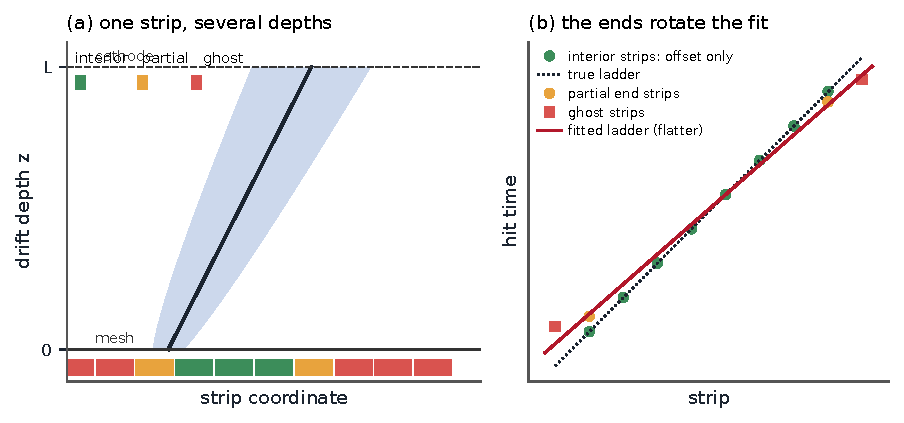
\includegraphics[width=\linewidth]{schematic}
  \caption{(a) A strip reads the charge of several drift depths: the interior strips (green) collect a full box of depths, the
  two partial strips at the ends of the column (orange) a fraction of one, and the ghost strips (red) only what the lateral
  spread (shaded) brings them. (b) In the ladder of one time per strip, the interior strips keep the true slope and move
  together; the partial strips and the ghosts are displaced in opposite directions at the two ends and rotate the fitted
  line toward a steeper track.}
  \label{fig:schematic}
\end{figure}

\section{What spreads the charge, and what separates the mechanisms}\label{sec:mechanisms}

The literature uses ``capacitive coupling'' for several different processes, and a citation for one does not support another.
\Cref{tab:mechanisms} lists the processes that put charge of one depth on a neighbouring strip, with the time structure and the
dependences that distinguish them. The last two columns are the ones that matter for the $\mu$TPC: whether the share depends on
the drift depth, and whether it depends on where within the strip the charge lands.

\begin{table}[t]
  \centering\footnotesize
  \caption{Processes that put charge of one depth on a neighbouring strip. ``Same time'' means the neighbour's signal has the
  time structure of the strip's own charge. The MX17 column gives the values measured or bounded in \cref{sec:measurements}.}
  \label{tab:mechanisms}
  \begin{tabular}{@{}p{2.9cm}p{3.3cm}p{1.9cm}p{1.7cm}p{1.7cm}p{2.9cm}@{}}
    \toprule
    Process & Physics & Time on the neighbour & Depth dependence & Position-in-strip dependence & MX17 (chamber A) \\
    \midrule
    Drift diffusion & Gaussian, $\sigma^2 = D_T^2 z$ & same time & grows as $\sqrt{z}$ & yes & $D_T \approx \SI{350}{\micro\metre\per\sqrt{cm}}$, $\sigma_T(L) \approx \SI{0.6}{mm}$ \\
    Prompt footprint & avalanche spread, charge equalisation across the resistive strip width, induction through the insulator & same time & none & yes, smooth & Gaussian-equivalent \SIrange{0.33}{0.37}{mm} (X), narrower (Y) \\
    Floating-electrode imaging & charge on the resistive strip images onto several readout electrodes in the ratio of capacitances & same time, same shape & none & none (fixed ratio) & $\lesssim 7\,\%$ per side on X, bounded by the phase test \\
    Direct inter-strip capacitance & strip-to-strip $C$ into a charge amplifier: a transient leading the main pulse & derivative-like, leads by \SIrange{40}{115}{ns} & none & none & not required by the waveforms (derivative term $<$ a few \% per sample) \\
    Front-end or connector cross-talk & mutual capacitance in the ASIC or flex & same time or derivative & none & none & second neighbour \SI{1.3}{\%} within a chip, \SI{0.45}{\%} across a boundary (X) \\
    Resistive spreading along the strip & 1-D RC line, $\sigma^2 = 2 D_{RC} s$ with $s$ the time since landing & delayed and longer & grows with time since landing & yes & $D_{RC} = \SI{3.8e-4}{mm^2/ns}$ on Y; none across the strips \\
    Weighting-field induction & Shockley--Ramo current on a non-collecting strip & bipolar, zero net & none & yes & $\approx 0$ after shaping \\
    \bottomrule
  \end{tabular}
\end{table}

For the angle bias the table has one message: the first five rows all feed the end strips with same-time charge, and the
ladder cannot tell them apart. Within the forward model of \cref{sec:measurements} the total compression is invariant as the
same-time share is moved between a Gaussian footprint and a nearest-neighbour coupling kernel along the valley of equal
waveform $\chi^2$~\cite{paperII}: a fixed fraction $\kappa$ on both neighbours and a Gaussian of width $\sigma_0$ add to the cluster
variance alike ($\sigma^2 \to \sigma^2 + 2\kappa p^2$), and it is the variance that sets the ghost strips. What distinguishes the
processes is therefore not the bias but three other observables:

\begin{description}
\item[Depth.] Diffusion grows as $\sqrt{z}$; resistive spreading grows with the time since landing; every same-time coupling
  is the same at every depth. On near-normal tracks, where the column stays within a fraction of a pitch, the neighbour share
  read sample by sample against the drift time separates the constant part (the same-time share at the mesh) from the growing
  part, and the growth measures $D_T$ (\cref{sec:depth}).
\item[Position in the strip.] A Gaussian footprint puts most of its share on the neighbour nearer to the charge and little on
  the far one; a fixed coupling puts the same fraction on both. The far neighbour's share as a function of the charge's
  position within the strip therefore bounds the coupling (\cref{sec:phase}). The test is only as good as the position
  estimate, which in a $\mu$TPC comes from the same waveforms; \cref{sec:phase} includes its closure.
\item[Delay.] Resistive spreading arrives later and lasts longer, which is how the T2K ERAM analysis separates its ``charge
  spreading'' from diffusion's ``charge sharing''~\cite{T2K2022}. The delay separates the RC term from everything else, and
  nothing else: a same-time coupling and a same-time footprint sit on the same side of it.
\end{description}

A fourth observable, the channel map, separates electronics from the board: cross-talk inside a front-end chip or a connector
follows channel adjacency, charge sharing on the board follows strip adjacency, and the two differ at chip and connector
boundaries (\cref{sec:phase}).

The sizes in the literature for ``the'' coupling fraction, \SIrange{5}{67}{\%}~\cite{Farinelli2019,Ntekas2016,Loesel2017,Scholer2021},
are not one quantity. The 5\,\% is a pulse injected into a GEM strip and read on the neighbour after about \SI{15}{ns}
\cite{Farinelli2019}; the 10 to 15\,\% are a circuit simulation and an edge-strip charge correlation on one ATLAS test chamber
\cite{Ntekas2016}; the 23 to 32\,\% are an LTspice model of resistive strips 10 to 150~cm long~\cite{Loesel2017}, afterwards
adopted as a correction factor~\cite{Flierl2018,Herrmann2019}; the 67\,\% is the peak of an edge-to-inner charge ratio on the
longest NSW strips read with the VMM, which assumes the edge strip is pure coupling~\cite{Scholer2021}. A factor tuned to
restore the angle, such as the 20 or 30\,\% of~\cite{Flierl2018,Herrmann2019}, absorbs every same-time share, diffusion and
footprint included, and measures no capacitance.

\section{What the detector families have reported}\label{sec:literature}

\Cref{tab:families} places the families on the two numbers of \cref{sec:scaling}. The first column group is the geometry, the
last three are what was reported and how it was handled. All lever arms are derived from the published geometry and
diffusion coefficients, since no source states the quantity; where a diffusion coefficient had to be assumed it is marked.

\begin{table}[t]
  \centering\footnotesize
  \caption{Detector families against the two numbers that control the single-time bias: the strips in a full-drift column at
  $\tan\theta = 0.3$ and the transverse diffusion at full drift in units of the pitch. $\Lambda_{0.3} = \sigma_T(L)/(L\tan\theta)$
  is the lever arm. Derived values rest on the cited geometry; the LMU diffusion coefficients are assumed equal to the NSW value.}
  \label{tab:families}
  \begin{tabular}{@{}p{3.1cm}cccc>{\raggedright\arraybackslash}p{3.0cm}>{\raggedright\arraybackslash}p{2.9cm}@{}}
    \toprule
    Family (examples) & $L$ [mm] & $p$ [mm] & $N_{0.3}$ & $\sigma_T(L)/p$ & Time estimator; reported bias & Treatment \\
    \midrule
    MX17 chamber A (this work) & 28 & 0.78 & 10.8 & 0.75 & leading edge, peak, template, centroid: ratio 1.19 (X), 1.37 (Y) at the sample median & forward fit of the waveforms \\
    ATLAS NSW Micromegas~\cite{Iodice2015,Ntekas2016,Scholer2021} & 5 & 0.425--0.45 & 3.4 & 0.6 & APV25 rise time, VMM peak; \ang{20}$\to$\ang{23}; sharing-off simulation still $+\ang{7}$ & edge filters, position polynomial, angle cuts \\
    LMU floating strip~\cite{Bortfeldt2014,Bortfeldt2015} & 6 & 0.5 & 3.6 & 0.56 & Fermi fit; \ang{10}$\to$\ang{15} measured, \ang{19} in LTspice & angle-dependent rescale \\
    LMU GEM~\cite{Flierl2018} & 8 & 0.4 & 6 & 0.82 & Fermi fit; \ang{15}$\to$\ang{19}, \ang{30}$\to$\ang{32} & 15--20\,\% neighbour subtraction \\
    BESIII CGEM~\cite{Alexeev2019,Farinelli2019} & 5 & 0.65 & 2.3 & 0.38 & APV25; ``tilt towards larger angles'' & edge weighting, \SI{180}{\micro\metre} shift \\
    T2K ERAM~\cite{T2K2022,T2K2023} & 970 & 10--11 & 27 & 0.3 & time of maximum; RC delay, no angle bias reported & RC and gain maps; no time ladder \\
    ALICE, STAR pad TPCs~\cite{Alme2010,Anderson2003} & 2100--2500 & 5--7 & 110 & 0.6--0.9 & charge-weighted time per row; resolution terms only & drift scale from lasers and silicon \\
    LArTPCs~\cite{Adams2018a,Adams2018b,ProtoDUNE2020,ICARUS2024} & 1500--3600 & 3--4.8 & 230 & 0.3--0.8 & Gaussian peak after 2-D deconvolution; width and charge vs angle, no time bias found & deconvolution in wire and time \\
    Directional and short-track TPCs~\cite{MIMAC2020,BEAST2019,MAIKo2018} & 10--250 & 0.05--2 & few & 0.5--8 & threshold, TOT midpoint, slice barycentre; ``canoe'' shapes, slice ends deviate & none; resolution \ang{1}--\ang{60} \\
    GridPix~\cite{GridPix2018} & 20 & 0.055 & 110 & 8 & time of each electron & nothing to aggregate \\
    \bottomrule
  \end{tabular}
\end{table}

\subsection{Strip micro-TPCs: the bias is a family trait}

Every strip $\mu$TPC that published a comparison with a set angle reports the track too steep, with the excess shrinking as
the angle grows. Bortfeldt measured $+\ang{5}$ at \ang{10} on a floating-strip Micromegas and predicted $+\ang{9}$ with a
parameter-free LTspice model of the strip capacitances, which also reproduced the fall with angle (\ang{4.3}, \ang{2.0}, \ang{0.6}
at \ang{20}, \ang{30}, \ang{40})~\cite{Bortfeldt2014}; the journal version names two effects, ``signals couple capacitively onto
neighboring strips'' so that ``measured signal timing is shifted towards earlier values for the strips hit by electrons created
close to the cathode'', and ``for strips at the edges of the strip cluster, the ionization electrons position is not calculated
correctly''~\cite{Bortfeldt2015}. ATLAS test chambers at \ang{20} peak near \ang{23}~\cite{Iodice2015}, ``understood to be due to
the capacitive induction of the signal on neighboring strips'', a formulation the BESIII GEM papers repeat nearly verbatim while
adding that ``the transverse diffusion plays another important role''~\cite{Alexeev2019}. Flierl's GEM read \ang{19} (most probable)
at \ang{15} and \ang{32} (mean) at \ang{30}~\cite{Flierl2018}. In the units of \cref{eq:scaling} these are tan ratios of 1.52, 1.17, 1.28
and 1.08 at $N$ of 2.1, 4.5, 5.4 and 11.5 (\cref{fig:universal}b), and $(\text{ratio}-1)N^2$ lies between 2 and 11 for all of
them.

The attribution rests on two roots, Bortfeldt's circuit model~\cite{Bortfeldt2014} and the NTUA/ATLAS Maxwell--Simplorer model
with an edge-strip charge correlation~\cite{Ntekas2016}; later papers cite or restate them~\cite{Sessa2014,Vanadia2015,Rinnagel2019,Alexeev2019,Farinelli2019}.
Neither root excludes the alternatives. Bortfeldt's model has coupling and the edge-position effect but no diffusion, and
gives no decomposition; Ntekas's thesis states that the gas-only Monte Carlo ``without the fully equivalent electrical circuit''
still shows a bias, ``purely geometrical coming from the incomplete overlap of the outer cluster strips with the particle's
trace inside the MM gas gap combined with the diffusion of the ionisation electrons'', of \ang{0.2} at \ang{30} rising to \ang{4} at
\ang{10}~\cite{Ntekas2016}. Scholer's NSW digitisation, with diffusion on and charge sharing switched off, peaks \ang{7} high for
tracks above \ang{25}, an offset he attributes to ``the positions of the first and last ionizations above the corresponding
strips'' and leaves to ``further investigation''; with sharing on the peak moves higher, and his own test beam at \ang{28} shows no
shift at all~\cite{Scholer2021}. That test beam is the one published measurement that lies below the no-coupling
toy of \cref{app:toy}, which on the NSW-like geometry with the VMM peak time gives a tangent ratio of 1.10 at \ang{28}, a
peak about \ang{2} high; his own simulation, \ang{7} high, misses it by more. Two differences are not checked: the quoted value is
the peak of a distribution with a long tail towards larger angles (resolution \ang{7.1} about the peak), not the median our
ratios use, and a $6\times$ r.m.s.\ threshold that drops the faint end strips acts as an edge cut (\cref{sec:remedies}).
Klitzner, with floating strips in the fast gas Ne:CF$_4$, finds the angle too large at drift fields below 300~V/cm, but
on one layer only: ``all other layers reconstruct a slightly smaller angle than expected''~\cite{Klitzner2016}. These are
the two published cases where the bias is absent or reversed; neither author explains them, and we cannot either. Herrmann, on a full-size NSW module, adopts a 30\,\% coupling correction from Lösel's
simulation~\cite{Loesel2017} and Flierl's analysis, and states the mechanism in strip-count terms: without the correction ``no
mean-time difference is in the range expected from the drift velocity'', and ``the time difference is biased for lower
inclination due to the low number of affected strips''~\cite{Herrmann2019}. The only other mechanism statement we found is a
2024 conference poster by Fang et al., who derive a per-strip time correction from transverse and longitudinal diffusion on the
argument that the first of several primary electrons sets the strip time~\cite{Fang2024}; it concerns the segment midpoint and
has no journal version.

Two facts stand out. No source varied one parameter and tracked the bias: pitch, strip length, drift field and electronics are
confounded in every comparison, and a drift-field scan changes the diffusion, the velocity, the time per strip and the signal
to noise together. And no source had a per-track external angle; the set angle of a chamber is known to about a degree, which at
\ang{10} is 10\,\% in the tangent, the size of the effect under study.

\subsection{Pad TPCs and liquid-argon TPCs: the same spread, a longer column, another estimator}

The large pad TPCs have a transverse diffusion at full drift comparable to their pad width (ALICE 0.6--0.9, STAR 0.5--1.0 in
units of the pad~\cite{Alme2010,Anderson2003}), the same as MX17's 0.75. What differs is the column: 45 to 150 rows against 3
to 13 strips, so the end strips are a fraction of a per cent of the points. They also read a charge-weighted time, STAR
``weighting the average by the amount of charge collected in each bucket''~\cite{Anderson2003} and ALICE a centre of gravity over
time bins~\cite{Alme2010}, which has no interior compression. Their angle-dependent terms (the angular pad and angular wire effects,
$\tan^2\alpha$ in the resolution, threshold losses) are variances, not slope biases, and their drift scale is fixed by lasers
and silicon to 0.1\,\%. A multiplicative compression of the drift coordinate would be absorbed into the effective drift
velocity by a track-based calibration~\cite{Alme2010}; at the 0.1\,\% our scaling predicts for a 1.3~m column there is nothing to
absorb.

The liquid-argon TPCs are the closest relatives of the forward model. MicroBooNE writes the wire signal as the charge
convolved with a field and electronics response in wire and time and solves it as a two-dimensional deconvolution, with
Wiener-type filters, because the long-range induction puts a signal on wires that collect nothing~\cite{Adams2018a,Adams2018b};
ProtoDUNE-SP uses the same form~\cite{ProtoDUNE2020}. Their kernel is the induced current, bipolar and calculated; the transverse
diffusion stays in the deconvolved image. MicroBooNE states the mechanism for the pulse width, adjacent clouds that ``begin to
overlap as they spread in the $yz$-plane under the influence of $D_T$, causing additional $\sigma_t$ smearing'' that grows with the
angle to the wire plane~\cite{MicroBooNE2021}, and ICARUS tunes its wire response in angle bins~\cite{ICARUS2024}. A bias of the
hit time or of the local slope has not been reported; with columns of hundreds of wires it would be below a per mille, and a
3~cm segment at full drift, where the lever arm is as short as MX17's, has not been tested against an external slope.

\subsection{Directional and short-track detectors: the column but no reference}

The keV-to-MeV recoil detectors have short tracks on fine channels and one time per channel (NEWAGE, BEAST, D3, MAIKo,
MIGDAL's strip plane), or a barycentre per time slice (MIMAC, ACTAR)~\cite{MIMAC2020,BEAST2019,MAIKo2018,MIGDAL2023}. Two of them
describe the artefact without quantifying it: BEAST's pixel tracks take a ``canoe shape'' because ``the pixel integration time
is longer than the typical charge cloud size''~\cite{BEAST2019}, and MIMAC's ``initial and final time slices of the track
usually have a larger than average deviation from the track direction''~\cite{MIMAC2020}. Their angle references are
kinematics at \ang{10} to \ang{16} resolution, source pointing with no absolute drift coordinate, or the self-consistency of the two
halves of one track, which a common scale error passes. A few per cent of slope is invisible to all of them. The single-electron
pixel detectors (GridPix) have nothing to aggregate and report only a time walk~\cite{GridPix2018}; their drift scale is
calibrated with a telescope, which would absorb a compression~\cite{GasPix2019}.

\subsection{Drift tubes: the one time per wire is already a functional of the inclination}

The oldest time-projection readout shows the general statement in another guise. The drift time of a wire is the arrival of
the first electrons from the track segment seen by that cell, and its relation to the distance of closest approach depends on
the track's inclination to the cell: the CMS drift tubes calibrate a maximum drift time that ``depends on the track inclination
and on the pattern of cells crossed'' and an effective drift velocity that depends on ``the inclination of the
track''~\cite{CMSDT2010}; the BESIII drift chamber determines separate space-time relations ``for 10 degree steps'' of the entrance
angle because the differences ``grow with the increasing drift times up to as much as several hundred microns''~\cite{BESIIIMDC2014};
Belle II parametrises its relations per layer, side and angle category~\cite{BelleIICDC2019}. These detectors never see the
problem as a bias because the angle-dependent calibration is part of the method. The $\mu$TPC has no such calibration, because
its purpose is to measure the inclination that the calibration would have to know.

\subsection{What survives the survey}

A transparent toy with drift diffusion, the strip geometry and a small induction footprint, and no coupling of any kind,
reproduces the published biases of the NSW-type, floating-strip and GEM chambers to within a factor 1.6 in the excess
$\tan\theta_{\rm rec}/\tan\theta - 1$ on the four measured points (toy over published 1.6, 1.3, 0.8 and 0.6, \cref{tab:toydet}), with no
free parameter beyond an assumed footprint and diffusion; the circuit model's predictions at \ang{20} to \ang{40} and the diffusion-only toy differ by
less than 0.05 in the tangent ratio. The angle, in other words, never contained the information that would have identified
the coupling.

The bias is not new, the model equation is not new, and the per-channel waveform fit has relatives in T2K's RC maps and in the
LArTPC deconvolution. What had not been done is to measure the compression per track against an independent reference, to
separate the geometric end term from the lateral spreads and the spreads from each other, and to fit the drift-depth charge
profile of each track inside the convolution model. Those are the contributions of \cref{sec:measurements,sec:remedies}, and the
companion paper~\cite{paperII}.

\section{Measurements on a deep resistive-strip micro-TPC}\label{sec:measurements}

\subsection{The test bed}

The chamber is a bulk Micromegas with a \SI{28.08}{mm} drift gap, 400~mm square, read by 512+512 strips of \SI{0.78}{mm}
pitch formed as combs of pads under a layer of resistive strips that run along the Y strips~\cite{paperI}. Both views are
sampled every \SI{60}{ns} by DREAM front-end chips, 32 samples per channel, so every strip's waveform is available offline. The
gas is Ar/iC$_4$H$_{10}$ 95/5 with about 1\,\% water at a drift field of \SI{350}{V/cm}, giving a drift velocity of
\SI{35.8}{\micro\metre/ns} from the column duration and \SI{37.1}{\micro\metre/ns} (X) and \SI{36.3}{\micro\metre/ns} (Y) from the
angle scale against the reference~\cite{paperI}; the full column lasts \SI{784}{ns} and spans $N = 36\tan\theta$ strips. Cosmic
muons are triggered by scintillators and tracked by a four-plane silicon telescope (M3) that gives each track's slope to
\SI{0.3}{mm} over \SI{1.3}{m}, so the reference angle is independent of the chamber and known per track. Two runs on the same
chamber on consecutive nights give 12\,366 and 38\,364 single-track projections (an X and a Y projection per track) with a
reference angle and a successful waveform fit~\cite{paperII}.

Two readings of every projection are compared with the reference. The hit reading emulates a hit-based front end on the
stored waveforms: a strip fires when a five-sample boxcar exceeds five times its noise, its time is the 30\,\% leading edge of
the pulse (the production definition), and the angle is the amplitude-weighted straight line through the hits. Alternative
estimators (time of the peak, template fit, charge-weighted mean, time over threshold, Fermi-Dirac rise) are emulated on the
same samples; their logic is that of the VMM, TIGER, APV25 or SAMPA chips, at the DREAM shaping. The waveform reading is a
per-event forward fit of every sample of every strip to \cref{eq:waveform} with a measured impulse response, a Gaussian
footprint $\sigma_0 = \SI{0.30}{mm}$, drift diffusion $D_p = \SI{0.023}{mm/\sqrt{ns}}$ (equivalent to
$D_T \approx \SI{385}{\micro\metre\per\sqrt{cm}}$) and, on the Y view, resistive spreading with $D_{RC} = \SI{3.8e-4}{mm^2/ns}$; the
charge of each \SI{60}{ns} depth slice is a free non-negative parameter and the track parameters $(x_0, w, t_0)$ are
searched~\cite{paperII}. Its angle scale is calibrated on the reference ($k_w = 1.037$ on X, 1.015 on Y); after that calibration
it reads the reference slope to within 1\,\% at every angle (\cref{fig:universal}a, W).

The same model regenerates each projection's waveforms with its own fitted track and charge profile and with one ingredient
changed, and the real residual (data minus fit) added back, so that the hit emulators can be run on windows whose truth is
known exactly~\cite{paperII}. We use the arms: \emph{base} (the model as fitted), \emph{metallic} (footprint reduced to the
\SI{0.07}{mm} induction floor and no resistive term, what a metallic readout in the same gas would show), \emph{no diffusion}, \emph{geometry only}
(no diffusion, floor footprint, no resistive term: the strip width alone) and a footprint of \SI{0.45}{mm}. The residual carries
the real noise and whatever the model does not describe, so these arms include the data's unmodelled components; a
transparent toy with white noise and the same template (\cref{app:toy}) gives the clean physics.

\subsection{The compression is a strip-end effect}\label{sec:ratio}

\Cref{fig:universal} shows the median ratio $\tan\theta_{\rm hits}/\tan\theta_{\rm ref}$ against the reference angle for the
leading-edge hits of Run 1 and against $N$. The ratio is 4.2 at $|\tan\theta| = 0.04$, 1.55 at 0.10, 1.24 at 0.15, 1.115 at
0.22 and 1.02 at 0.35 on X, and 6.4, 1.89, 1.35, 1.17 and 1.06 on Y; Run 2 agrees within 0.02 at every angle. The fit
$\Delta\tan\theta = a/\tan\theta + b\tan\theta$ gives
\begin{align*}
  \text{X:}\quad a &= 0.0054\ (\text{Run 1}),\ 0.0056\ (\text{Run 2}), & b &= -0.003,\ +0.017, \\
  \text{Y:}\quad a &= 0.0090,\ 0.0088, & b &= -0.019,\ +0.002,
\end{align*}
i.e.\ $C = a(L/p)^2 = 7.0$ to $7.3$ on X and $11.4$ to $11.7$ on Y, and an interior term consistent with zero at the
$\pm 0.02$ level once the data are put on the calibrated angle scale (with the timing velocity instead, every ratio is inflated by
$k_w - 1$ and $b$ reads $+0.03$ to $+0.05$: a drift-velocity error is indistinguishable from an interior compression, which is why
a $\mu$TPC cannot calibrate its own drift velocity from the ladder). The $1/N^2$ form is the one of \cref{eq:scaling}: on the
log--log plot of \cref{fig:universal}b the data lie on a line of slope $-2$ from $N = 1.4$ to $N = 13$. At the sample median,
$|\tan\theta| \approx 0.11$ and $N \approx 4$, the ratio is 1.5 and the angle reads \ang{2.5} to \ang{3} too steep.

The arms decompose $C$ (\cref{tab:arms}). Geometry alone, the partial strips of the strip width with a point-like footprint and
no diffusion, gives $C = 2.3$; the \SI{0.30}{mm} footprint raises it to 3.8; diffusion with the floor footprint gives 5.4; both
together give 6.9, the data's 7.0 on X. On Y the resistive spreading adds 4.6 more ($C = 11.5$ against the data's 11.7); with
twice the spreading constant $C$ would be 17. The same ingredients in the white-noise toy give 1.3, 2.8, 4.3 and 6.0
(\cref{app:toy}): each ingredient contributes the same increment, and the arms sit about one unit above the toy because they
carry the real residual (\cref{sec:ghosts}).

\begin{table}[t]
  \centering\small
  \caption{The strip-end coefficient $C$ (ratio $-1 = C/N^2$) for the leading-edge hits: data against the reference, model
  arms with exact truth and the real residual, and the white-noise toy. The interior term $b$ is given for the data; it is
  $-0.01$ to $-0.02$ for every arm (a \SI{60}{ns} depth-quantisation artefact of the arms at steep angles) and $+0.005$ to
  $+0.008$ in the toy.}
  \label{tab:arms}
  \begin{tabular}{@{}llccc@{}}
    \toprule
    & & $C$ (arms) & $C$ (toy) & data $C$, $b$ \\
    \midrule
    X & geometry only (strip width) & 2.3 & 1.3 & \\
      & + footprint \SI{0.30}{mm}, no diffusion & 3.8 & 2.8 & \\
      & + diffusion, floor footprint (``metallic'') & 5.4 & 4.3 & \\
      & footprint + diffusion (model) & 6.9 & 6.0 (6.5 at $D_p = 0.023$) & $7.0$--$7.3$, $b = -0.003/+0.017$ \\
      & footprint \SI{0.45}{mm} + diffusion & 9.1 & 8.0 & \\
    Y & model without resistive spreading & 7.3 & & \\
      & model (with $D_{RC}$) & 11.5 & & $11.4$--$11.7$, $b = -0.019/+0.002$ \\
      & $2\times D_{RC}$ & 16.8 & & \\
    \bottomrule
  \end{tabular}
\end{table}

The estimator does not change the picture. On the same planes the template-fit time (a matched filter, the best single time a
strip can give) reads $C = 6.7$, the Fermi-Dirac rise 6.1, the peak time 7.2 and the threshold crossing 9.5 on X
(\cref{tab:remedies}); the charge-weighted time, which the toy predicts to remove the interior term, reads 7.8 and is no
better than the leading edge, because there is no interior term to remove. Nor does the pitch: summing adjacent strips into
readout elements of $k$ pitches (\cref{fig:pitch}) raises $a$ from 0.0054 to 0.0075, 0.0108, 0.0161 and 0.030 for $k = 2, 3, 4, 6$
in the data, and the geometry-only arm follows ($0.0019 \to 0.0041, 0.0075, 0.0111$), so most of the growth is the strip-end
geometry itself. Fine strips are not the cause; coarser ones make it worse.

\begin{figure}[t]
  \centering
  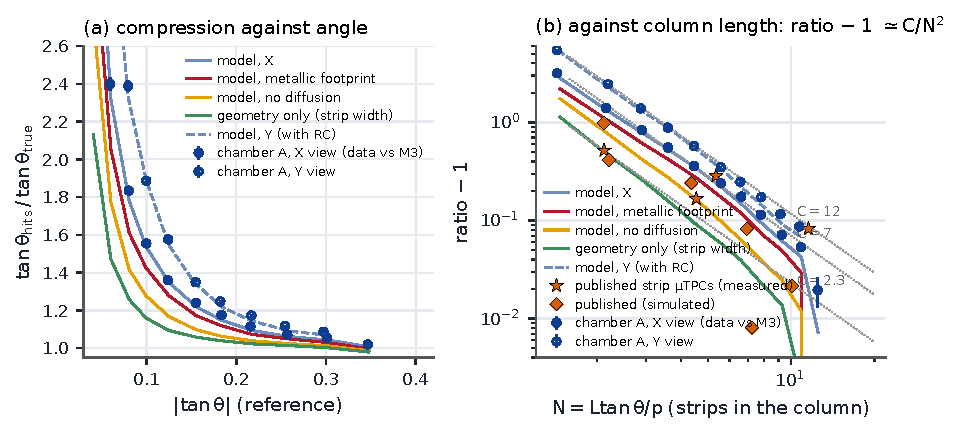
\includegraphics[width=\linewidth]{universal}
  \caption{(a) The median ratio of the hit-time angle to the reference angle against the reference angle, for the data of
  Run 1 (markers; filled X, open Y) and for the model arms (lines, exact truth). (b) The same as ratio $-1$ against the number of
  strips in the column, with the published strip-$\mu$TPC points converted from the quoted set and reconstructed angles with
  each chamber's gap and pitch (stars: measured; diamonds: circuit or gas-only simulations). Dotted lines: $C/N^2$ for $C = 2.3$
  (geometry), 7 (data X) and 12 (data Y).}
  \label{fig:universal}
\end{figure}

\begin{figure}[t]
  \centering
  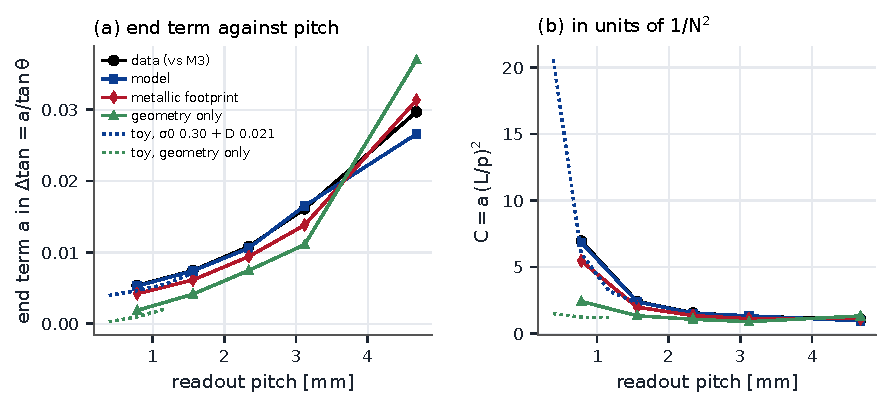
\includegraphics[width=\linewidth]{pitch_scan}
  \caption{The end term $a$ (left) and $C = a(L/p)^2$ (right) against the readout pitch, from summing adjacent strips of the
  same windows into readout elements of $k$ pitches; data against the reference, and the model arms. The toy (dotted) is the
  same scan with white noise.}
  \label{fig:pitch}
\end{figure}

The published points of \cref{fig:universal}b fall in the band spanned by the arms. Bortfeldt's measured \ang{10} point
($(\text{ratio}-1)N^2 = 2.3$) and Ntekas's gas-only simulation at \ang{10} (2.0) sit on the geometry line, Iodice's NSW chamber at
\ang{20} (3.4) and Bortfeldt's circuit model (3.9 to 4.7) between the geometry and the no-diffusion arms, and Flierl's GEM
(8.3 at \ang{15}, 10.8 at \ang{30}), whose diffusion at full drift is 0.8 of its pitch like ours, on the data line. The ordering follows
the lateral spread in units of the pitch, as \cref{eq:scaling} says it should; with diffusion coefficients assumed for the
LMU chambers and most-probable or mean angles quoted, this is a consistency check and not a measurement.

\subsection{Lateral sharing against drift depth}\label{sec:depth}

On tracks within \ang{0.5} of the drift direction ($|w| < \SI{3e-4}{mm/ns}$, so that the track moves less than a third of a pitch
over the gap) every sample of a strip's waveform belongs to a known drift time, smeared by the \SI{200}{ns} impulse response.
Stacking the waveforms of the five strips around the track at $t - t_0$ and dividing gives the neighbour shares against drift
depth (\cref{fig:depth}); the arms, regenerated on the same tracks and stacked the same way, carry the same smearing.

On the X view (569 planes) the first-neighbour share $(W_{-1} + W_{+1})/W_0$ is $0.50 \pm 0.02$ at $t_0$ and grows to 0.80 at
\SI{400}{ns} and $1.18 \pm 0.03$ at \SI{1000}{ns}. With the diffusion switched off the model's share is flat at 0.46 to 0.48: the growth
is drift diffusion, and its rate, read from the erf-fitted width of the five-strip pattern, is $d\sigma_{\rm eff}^2/dt =
\SI{3.5e-4}{mm^2/ns}$ against $4.2$ for the model's $D_p = 0.023$ and $3.2$ for $D_p = 0.020$: the data prefer $D_p \approx
\SI{0.021}{mm/\sqrt{ns}}$, $D_T \approx \SI{350}{\micro\metre\per\sqrt{cm}}$, 8\,\% below the fitted value and inside the Magboltz range for
this gas. The metallic arm starts at 0.27: without a same-time footprint of the model's size the mesh-end share is half the
data's, so a same-time share is required at the mesh, equivalent in the width metric to a Gaussian of \SIrange{0.33}{0.37}{mm}
on X. On Y (744 planes) the first-neighbour share grows to 2.0 by \SI{800}{ns} and the resistive spreading supplies most of
the growth (the arm without it reaches only 1.1); the mesh-end share is lower than on X ($0.49$ against $0.50$ with a model
that puts $0.60$ there), i.e.\ the same-time footprint along the resistive strips is narrower than across them, as it should be
if the footprint across the strips includes the equalisation of the avalanche charge over the \SI{550}{\micro\metre} strip
width~\cite{paperII}.

The second neighbours tell a different story. At $t_0$ their share is $0.049 \pm 0.004$ on X and $0.047 \pm 0.001$ on Y, about
2.4\,\% per side, where any Gaussian footprint of the fitted width gives less than 0.01 and the model 0.006; the kernels fitted
with a same-time second-neighbour term ($k_2 = 0.01$ to $0.02$) reproduce it (0.044 and 0.061). At depth the data's second-neighbour
share also exceeds every arm (0.27 against 0.24 for the model at \SI{1000}{ns} on X): the lateral distribution of the collected charge
has heavier tails than a Gaussian, at the mesh and at the cathode. A channel-map test~\cite{paperII} assigns most of the
mesh-end second-neighbour share to the electronics (1.34\,\% within a chip against $0.45 \pm 0.11$\,\% across a chip or connector
boundary on X); the first-neighbour share does not change across boundaries and is a property of the board.

\begin{figure}[t]
  \centering
  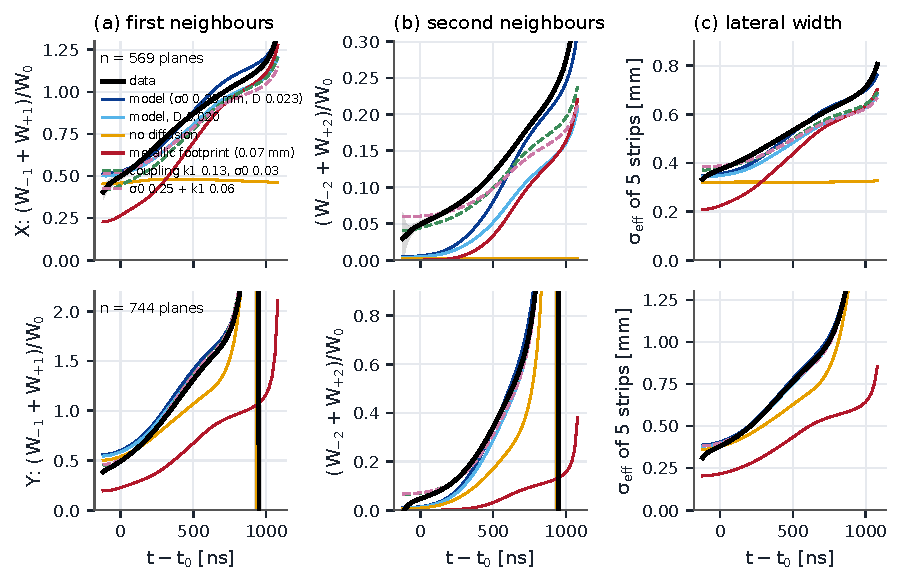
\includegraphics[width=\linewidth]{depth_sharing}
  \caption{Lateral sharing against drift depth on near-normal tracks ($|\tan\theta| < 0.008$), X (top) and Y (bottom): (a) the
  first-neighbour share, (b) the second-neighbour share, (c) the erf-fitted width of the five-strip pattern, all against the
  time after the mesh charge, for the data (black, with bootstrap band) and the model arms regenerated on the same tracks. The
  growth of (a) and (c) is drift diffusion (flat without it); the mesh-end values are the same-time share; the second neighbours
  at $t_0$ are a same-time floor that no Gaussian footprint produces.}
  \label{fig:depth}
\end{figure}

\subsection{Position in the strip: bounding a fixed coupling}\label{sec:phase}

A fixed nearest-neighbour coupling puts the same fraction on both neighbours wherever the charge lands in the strip; a Gaussian
footprint puts it on the nearer one. \Cref{fig:phase}a shows, at $t_0$ on the X view, the share of the neighbour on the side
the fitted track leans to (``near'') and of the other (``far'') in three bins of the track's position within the strip. Near
the centre the two are $0.37/0.22$; at the edge $0.84/0.10$. The Gaussian model reproduces the near side everywhere and the far
side near the centre, and under-predicts the far side at the edge (0.07 against $0.10 \pm 0.01$); a pure nearest-neighbour
coupling of 13\,\% with a \SI{33}{\micro\metre} footprint, the kernel that replaces $\sigma_0$ at equal waveform $\chi^2$, is too low on the
near side near the centre (0.33) and too high on the far side at the edge (0.13); a kernel with a \SI{0.25}{mm} footprint and a
6\,\% same-time term matches all three bins on both sides. On Y the data's far share at the edge (0.12) is below every model and
no same-time floor is required.

The phase is the fitted position, and a fit that leans towards the brighter neighbour could create a near/far asymmetry
in symmetric data. \Cref{fig:phase}b closes this on 2\,900 planes per view: windows regenerated with a known truth (a
\SI{0.32}{mm} Gaussian with no coupling, or the pure 13\,\% coupling with a \SI{33}{\micro\metre} footprint), fresh noise at the
strip's $\sigma$, and the track refitted with the production fitter exactly as for the data, are processed identically. The
refitted position scatters about the truth by \SI{0.007}{mm} (Gaussian truth) and \SI{0.07}{mm} (coupling truth), a tenth of
a pitch at most, and the near/far shares with the refitted and the true position agree within 0.01 in every bin; on the
pure-coupling truth the refit turns the symmetric $0.160/0.144$ of the centre bin into $0.174/0.138$, a lean that falls far short
of the data's $0.205/0.124$. The test is therefore sound. On X the data's far share is $0.124$ at the centre and then flat at
$0.060$ to $0.067$ from a quarter pitch outward, where the Gaussian truth falls from 0.167 to 0.040 and the pure coupling stays
at 0.13: the data have a floor, and it is half the published coupling. On Y the floor is $0.10$ against a Gaussian's 0.07 and the
coupling's 0.13, while the centre bin ($0.216/0.159$) lies below the Gaussian's $0.279/0.209$: the same-time footprint along the
resistive strips is narrower than the fitted \SI{0.28}{mm} with a floor on top. In both views the same-time share is a narrow core
plus a flat few-per-cent floor, the shape of the kernels fitted with a footprint and a same-time term ($\sigma_0 = \SI{0.25}{mm}$ with
$k_1 = 0.06$ on X; \SI{0.12}{mm} with $0.09$ on Y~\cite{paperII}). A fixed nearest-neighbour coupling on chamber A is thus bounded at
about 6\,\% (X) to 10\,\% (Y) per neighbour, a factor two to five below the 15 to 30\,\% of the strip-$\mu$TPC literature, and
consistent with the published fraction that a floating resistive strip images onto the adjacent readout column for this stack-up
($\sim 1\,\%$ per side~\cite{paperII}) only if a further same-time process is present. Its physical origin is not identified. For
the angle it does not matter: the floor's variance is what the ghost strips see, and the forward model carries it as part of
$\sigma_0$.

\begin{figure}[t]
  \centering
  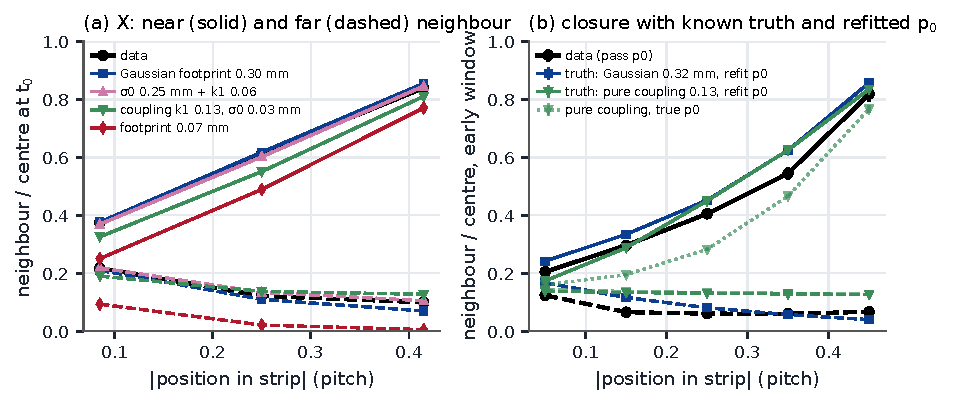
\includegraphics[width=\linewidth]{phase}
  \caption{(a) Near (solid) and far (dashed) neighbour share at $t_0$ on X against the track's position within the centre
  strip, data and models regenerated on the same tracks with the fitted position. (b) The closure: the same quantity on
  windows of known truth, with the track position refitted by the production fitter.}
  \label{fig:phase}
\end{figure}

\subsection{Ghost strips}\label{sec:ghosts}

The end effect lives in the strips beyond the column. Counting the strips with a hit whose centre lies more than half a
pitch outside the track's projection (\cref{fig:ghosts}), the data have 3.4 ghosts per plane on X at $|\tan\theta| = 0.08$--$0.15$
against 2.6 in the model with the same noise, and the excess is at the mesh end (1.57 against 0.82 per plane; the cathode end
agrees, 1.82 against 1.75). On Y the data have 5.5 ghosts per plane against 5.4 and the two ends agree within 0.3. The
mesh-end excess on X is the same-time floor of \cref{sec:depth} seen from the other side: charge that no Gaussian of the
fitted width brings to the second strip, at the earliest times, where it rotates the ladder most. It is the part of chamber
A's compression that the model does not describe, and the reason the arms with the real residual sit one unit of $C$ above
the toy.

\begin{figure}[t]
  \centering
  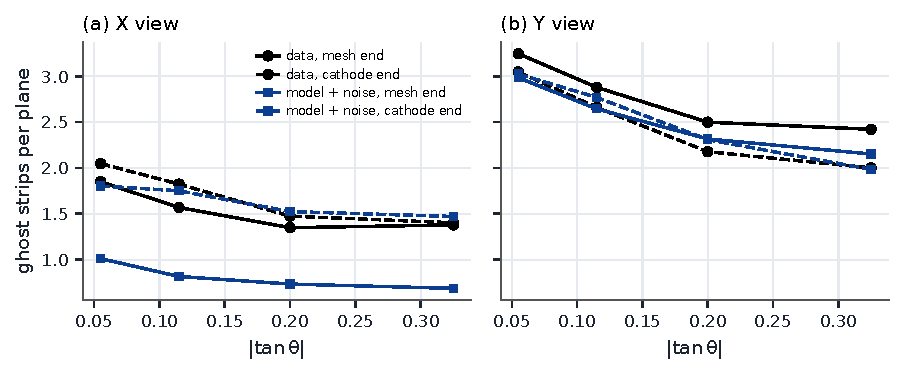
\includegraphics[width=0.8\linewidth]{ghosts}
  \caption{Ghost strips per plane (hits more than half a pitch beyond the track's projection), at the mesh end (solid) and the
  cathode end (dashed), data against the model with the same noise, Run 1.}
  \label{fig:ghosts}
\end{figure}

\section{Remedies, scored on the same tracks}\label{sec:remedies}

The literature's corrections were built for the end strips without saying so. We score each of them, and the charge-weighted
time, on the same 50\,000 projections against the reference, with two figures of merit: the median steepness bias in bins of
the reference angle (the median of the signed angle error times the sign of the reference angle, so that the compression does
not cancel between the two track directions) and the angle resolution $s_{68}$ (the 68th percentile of the absolute error about
the median within \ang{5}) after a global linear calibration of the slope on the other half of the events. The second figure is
what a $\mu$TPC with a calibration run achieves; the first is what it suffers without one. \Cref{tab:remedies} gives both for
Run 1; Run 2 agrees within 0.1 to 0.2 degrees throughout. The corrections are:

\begin{description}
\item[robust line] iterative $3\sigma$ trimming of strips about the line, the role of the Hough step in the NSW and APV25 chains;
\item[edge cut] the first or last strip dropped when its amplitude is below 1/2~\cite{Rinnagel2019}, 1/4 or 1/6~\cite{Sessa2014} of the
  inner neighbour's: the ghost-hit cut;
\item[edge shift] the kept edge strip moved inward by $(1 - a_{\rm edge}/a_{\rm inner})\,p/2$, the centroid of the partial column
  it collects: the geometric correction of Ntekas and Farinelli~\cite{Ntekas2016,Farinelli2019} in a form that needs no calibration;
\item[neighbour subtraction] $W_i \to W_i - f\,(W_{i-1} + W_{i+1})$ sample by sample before the hit is formed, with $f = 0.07$ (the
  same-time floor of \cref{sec:phase}), 0.15~\cite{Loesel2017,Flierl2018}, 0.20~\cite{Flierl2018} and 0.30~\cite{Herrmann2019};
\item[charge-weighted time] the centroid in time of the pulse above threshold, the estimator of the pad TPCs, which the formulation
  predicts to remove the interior term.
\end{description}

\begin{table}[t]
  \centering\footnotesize
  \caption{Hit-level remedies on chamber A, Run 1, against the reference: implied drift velocity of the raw ladder (true
  \SI{37.1}{} X / \SI{36.3}{\micro\metre/ns} Y), median steepness bias per angle bin without calibration, and the angle resolution
  after a global scale calibration. V0 is the leading-edge hit; ``template'' the per-strip matched-filter time; ``cw'' the
  charge-weighted time. H2c is the forward model of \cref{sec:forward} fitted to the hit lists; W the forward fit of the
  waveforms~\cite{paperII}.}
  \label{tab:remedies}
  \begin{tabular}{@{}llcccccc@{}}
    \toprule
    & & implied $v$ & \multicolumn{4}{c}{steepness bias [\si{\degree}] at $|\tan\theta|$ =} & $s_{68}$ [\si{\degree}] \\
    view & reading & [\si{\micro\metre/ns}] & 0.05--0.1 & 0.1--0.2 & 0.2--0.3 & 0.3--0.5 & calibrated \\
    \midrule
    X & V0 leading edge & 44.8 & 3.46 & 2.47 & 1.64 & 1.43 & 2.06 \\
      & V0 + robust line & 44.1 & 3.38 & 2.32 & 1.51 & 1.21 & 2.05 \\
      & V0 + edge cut 1/2 & 43.4 & 3.09 & 2.12 & 1.36 & 1.08 & 1.97 \\
      & V0 + edge cut 1/6 + edge shift & 43.6 & 3.16 & 2.16 & 1.42 & 1.15 & 1.97 \\
      & V0 + 15\,\% subtraction + robust & 41.1 & 2.40 & 1.46 & 0.96 & 0.76 & 1.69 \\
      & V0 + 15\,\% subtraction + edge shift & 40.3 & 2.02 & 1.25 & 0.82 & 0.74 & 1.54 \\
      & V0 + 30\,\% subtraction & 39.2 & 1.72 & 0.92 & 0.62 & 0.53 & 1.51 \\
      & charge-weighted time + robust & 44.9 & 3.61 & 2.48 & 1.59 & 1.23 & 2.26 \\
      & charge-weighted + 30\,\% subtraction & 38.6 & 1.69 & 0.69 & 0.39 & 0.48 & 1.60 \\
      & template time + 15\,\% + edge shift & 39.9 & 1.87 & 1.09 & 0.69 & 0.57 & 1.55 \\
      & H2c: forward model on hit lists & & \multicolumn{4}{c}{$-0.05$ overall} & 1.20 \\
      & W: forward fit of the waveforms & & $-0.02$ & $0.00$ & $-0.06$ & $+0.02$ & 1.04 \\
    \midrule
    Y & V0 leading edge & 51.5 & 4.18 & 3.21 & 1.98 & 1.40 & 2.68 \\
      & V0 + robust line & 47.2 & 3.85 & 2.50 & 1.43 & 0.94 & 2.42 \\
      & V0 + edge cut 1/2 & 46.8 & 3.71 & 2.40 & 1.36 & 0.87 & 2.40 \\
      & V0 + 15\,\% subtraction + robust & 42.8 & 2.69 & 1.48 & 0.78 & 0.38 & 1.98 \\
      & V0 + 30\,\% subtraction & 45.6 & 3.39 & 2.07 & 1.10 & 0.90 & 2.32 \\
      & charge-weighted time + robust & 47.6 & 3.09 & 1.96 & 1.09 & 0.80 & 2.66 \\
      & charge-weighted + 15\,\% + robust & 42.9 & 2.34 & 1.13 & 0.43 & 0.32 & 2.30 \\
      & template time + 15\,\% + edge shift & 41.9 & 2.28 & 1.16 & 0.47 & 0.21 & 2.02 \\
      & H2c: forward model on hit lists & & \multicolumn{4}{c}{$+0.19$ overall} & 1.28 \\
      & W: forward fit of the waveforms & & $+0.03$ & $0.00$ & $+0.05$ & $+0.04$ & 1.01 \\
    \bottomrule
  \end{tabular}
\end{table}

\begin{figure}[t]
  \centering
  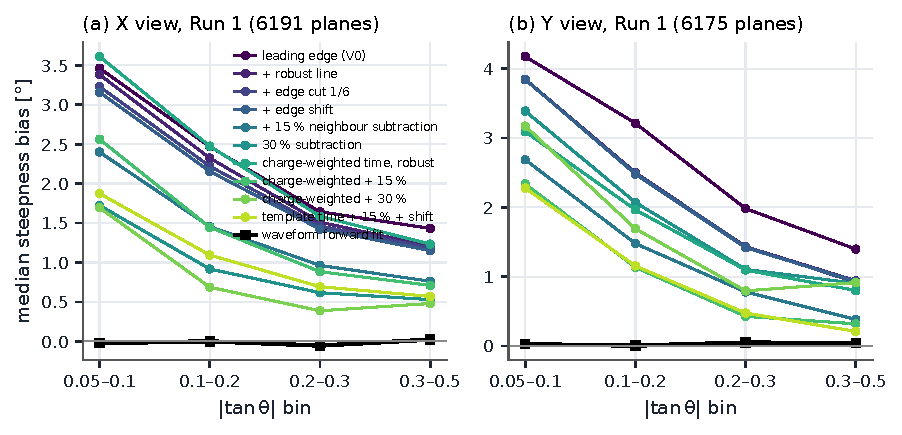
\includegraphics[width=\linewidth]{remedies_bias}
  \caption{Median steepness bias against the reference angle for the leading-edge hits with each correction, the
  charge-weighted time, and the forward fit of the waveforms (black), Run 1, X (a) and Y (b).}
  \label{fig:remedies}
\end{figure}

Four things follow (\cref{fig:remedies}).

\emph{The edge treatments act where the bias is and remove a quarter of it.} Cutting or shifting the edge strips lowers the
raw bias by 10 to 15\,\% at every angle on X and brings the calibrated resolution from \ang{2.06} to \ang{1.97}; the toy
(\cref{app:toy}) predicts a 24\,\% reduction of $C$ from the edge shift alone, with the difference made up by the real
chamber's ghosts, which the charge-ratio cut does not catch when they carry a few per cent of the centre strip at the
same time as it.

\emph{The neighbour subtraction is the strongest single correction, and its best factor is not a capacitance.} Subtracting
15\,\% of the neighbours' samples halves the calibrated resolution gap on X (\ang{1.69}) and Y (\ang{1.98}); 30\,\% does better on X
(\ang{1.51}, bias 0.5 to \ang{1.7}) but worse on Y (\ang{2.32}), where the neighbours' signals are the delayed resistive charge and
subtracting them at the same time removes real charge. The factor that restores the angle on X, 30\,\%, is Flierl's and
Herrmann's~\cite{Flierl2018,Herrmann2019}, and it is four to five times the same-time coupling that the waveforms allow
(\cref{sec:phase}): it deconvolves every same-time share in the ladder, the Gaussian footprint and the diffusion included, and
compensates the rest by over-correction. Herrmann's observation that even 40\,\% does not restore the expected first-to-last
time difference~\cite{Herrmann2019} is what one expects of a nearest-neighbour subtraction applied to a spread that reaches the
second neighbour and grows with depth.

\emph{The charge-weighted time does nothing by itself.} It reads the same compression as the leading edge on X (\ang{2.52} against
\ang{2.48} raw) and a worse one on Y (\ang{3.05}), where the delayed resistive charge pulls a centroid later on the strips it
reaches. It becomes the best estimator only after the subtraction (\ang{1.78} raw, \ang{1.28} on Y with 15\,\%), because the
subtraction removes the end charge and leaves an interior that the centroid reads without compression. The prediction of
\cref{sec:formulation} holds, and it is a statement about the interior term, which here is small.

\emph{No hit-level recipe closes the gap to the waveform fit.} The best combination on each view, 30\,\% subtraction on X and
charge-weighted time with 15\,\% subtraction on Y, leaves the calibrated resolution at \ang{1.5} to \ang{2.0} against \ang{1.0} for the
forward fit of the waveforms, and a residual bias of \ang{0.5} to \ang{2.3} without a calibration run. The forward model fitted
to the hit lists alone (H2c, one time and one amplitude per strip, the physics of the waveform fit and nothing of its
samples~\cite{paperII}) reaches \ang{1.20}/\ang{1.28}: most of the remaining gap is information the hits do not keep, not
knowledge the corrections lack.

\subsection{The forward model}\label{sec:forward}

The alternative to correcting the hit times is not to form them. \Cref{eq:waveform} is linear in the charge profile $q(u)$ for
a given track, so with the lateral spreads and the impulse response calibrated once per detector and run condition, the whole
strip-by-sample picture of an event can be predicted for a trial $(x_0, w, t_0)$ and the profile solved by non-negative least
squares; the track parameters are then the minimum of the $\chi^2$ over all samples of all strips~\cite{paperII}. The neighbours'
shares, same-time or delayed, are part of the prediction and stop being contamination; the partial strips and the ghosts are
predicted with the charge the model puts there and weigh in the fit by their information, not by a cut. The method is the
$\mu$TPC analogue of the simultaneous multi-pad waveform fit with which T2K maps its resistive spreading~\cite{T2K2023} and of
the channel-and-time convolution model of the liquid-argon deconvolution~\cite{Adams2018a}; what is new is that the drift-depth
profile is solved inside the fit, which is what turns a sharpened centroid into a track segment. On chamber A it reads the
reference slope to 1\,\% at every angle (\cref{fig:universal}a) with a resolution of \ang{1.0}, against a diffusion-limited floor of
\ang{0.3}~\cite{paperII}; on the re-simulated arms it stays within 1\,\% of the truth up to ten times the resistive spreading and for
every footprint and diffusion tried, because the mixing is in the model.

Its cost is the waveform: a sampled front end with enough samples to cover the column and the impulse response (here 32 at
\SI{60}{ns}), the calibration of the spreads per detector and run condition, and about a second of CPU per projection. A
hit-only front end that keeps one time and one amplitude per strip recovers most of the resolution gap only through the same
model (H2c), and none of it through corrections of the hit times.

\section{Consequences for design and analysis}\label{sec:guidance}

\paragraph{When will a readout see the bias?} \Cref{eq:scaling} with $C$ from \cref{tab:arms} answers it. For a leading-edge
or peak time and a lateral spread of 0.5 to 0.8 pitches at full drift, $C$ is 4 to 8, and the compression is 10\,\% at
$N \approx 7$ strips and 1\,\% at $N \approx 25$. A $\mu$TPC with a 5~mm gap and \SI{0.4}{mm} strips has $N = 12\tan\theta$ and
reads 1.3 at \ang{10}, 1.08 at \ang{20} and 1.02 at \ang{40}: the published curve. A pad TPC with a 1~m column and 1~cm pads has
$N = 100\tan\theta$ and a bias below $10^{-3}$ at every angle it measures; the same TPC reading a 3~cm segment near its anode
would see a few per cent. A readout that sums strips to save channels raises $C$ and lowers $N$ at once; in the pitch scan of
\cref{fig:pitch} doubling the pitch raised the end term by 40\,\% at fixed angle.

\paragraph{What the hit times cannot tell you.} The implied drift velocity of the raw ladder is not a drift velocity: on
chamber A it reads 45 and \SI{52}{\micro\metre/ns} for 37 and 36 (\cref{tab:remedies}), and every correction moves it. A
$\mu$TPC that takes $v$ from the ladder will read the right angle at one inclination and the wrong one everywhere else; one
that takes $v$ from the gas tables will read every angle too steep. A calibration against an external angle absorbs the
multiplicative part and leaves the $1/N^2$ part, which no constant can remove. The interior term and a drift-velocity error
have the same signature.

\paragraph{What to record.} The remedies of \cref{sec:remedies} rank the information: a time per strip gives the
compressed ladder; a time and an amplitude allow the edge treatments and the forward model on hit lists (\ang{1.2}); the samples
of the strips around the cluster allow the neighbour subtraction and the full forward fit (\ang{1.0}). Whatever is kept, the
neighbours of the cluster must be kept (the VMM's neighbour-enable logic does this), because the end strips are the
measurement of the spread and the model needs them. A threshold raised to suppress the ghosts removes the information that
locates the column ends.

\paragraph{How to separate the mechanisms.} The angle cannot; the compression is invariant under the exchange of a same-time
footprint for a same-time coupling of equal variance (\cref{sec:mechanisms}). Three measurements can, and each needs only
existing data: the neighbour share against drift depth on near-normal tracks (the constant is the same-time share, the growth is
diffusion, a delay is resistive spreading), the far-neighbour share against the position in the strip (a floor is a fixed
coupling, with its closure against the fitted position), and the channel map (electronics against board). The published
coupling fractions were obtained from none of these; a fraction tuned to restore the angle is a measure of the total same-time
spread, and should be reported as such.

\paragraph{What ``capacitive coupling'' should mean in the next paper.} On chamber A a same-time share of a few per cent per
neighbour is present, its second-neighbour part follows the channel map and is electronic, its first-neighbour part is on the
board and of unidentified origin, and its contribution to the angle bias is one of four of equal standing: strip geometry,
footprint, diffusion and (on the resistive view) RC spreading. A paper that attributes its $\mu$TPC bias to coupling should show
the depth and phase dependences that distinguish it from the other three, or call the whole same-time spread by one name.

\paragraph{What the forward model needs.} A measured impulse response per plane, the three spreads calibrated per detector and
run condition (they trade against each other in the waveform $\chi^2$, so the calibration must be anchored: the depth-resolved
stack fixes the diffusion and the mesh-end share independently of the fit), the drift velocity from the column duration, and
an angle scale from an external reference. With these it is unbiased at the per cent level and limited by diffusion and
ionisation statistics~\cite{paperII}. Without the reference it is still unbiased in shape, which the hits are not.

\section{Conclusions}\label{sec:conclusions}

The angle bias of single-time-per-channel track reconstruction, reported by every strip micro-TPC that compared itself with
a set angle and attributed to capacitive coupling, is a geometric property of reading a short drift column one time per
channel. A time per channel is a functional of the charge of every depth that reaches the channel; the channels at the two
ends of the column receive charge of the wrong depth from the partial overlap of the track with the strip and from any
lateral spread, and rotate the fitted line toward a steeper track. The ratio of the reconstructed to the true tangent is
$1 + C/N^2 + b$, with $N$ the strips in the column, $C$ set by the lateral spread in units of the pitch and the estimator, and
$b$ an interior compression from the growth of the spread with depth that is small for a leading edge and absent for a
charge-weighted time.

On a 28~mm resistive-strip Micromegas with a per-track silicon reference, $C = 7.0$ (X) and $11.7$ (Y) with $|b| < 0.02$; a
forward model of the waveforms reproduces $C$ to 2\,\% and decomposes it into strip geometry (2.3), the same-time footprint
(+1.5), drift diffusion (+3.1) and, across the resistive strips, RC spreading (+4.6); the published strip-$\mu$TPC points fall
between the geometry-only and the full curves in the order of their lateral spread; three further chambers, whose resistive
spreading constants span a factor three, reproduce the model's $C$ within 10\,\% on both views and order with the spreading
constant on the resistive view. Depth-resolved stacking of the strip
waveforms separates the same-time share at the mesh from a growth that matches a transverse diffusion of
\SI{350}{\micro\metre\per\sqrt{cm}}, and finds a same-time second-neighbour share of 2.4\,\% per side, mostly electronic, that no
Gaussian footprint gives. The position-in-strip test bounds a fixed nearest-neighbour coupling to about 6\,\% on the view
across the resistive strips, a factor three to five below the published fractions, and its closure shows the fitted position
to be adequate for the test. Nothing in the data requires a coupling of the published size, and nothing in the angle could
have told the difference.

The literature's remedies address the ends. Scored on the same tracks, the edge cuts and shifts remove a quarter of the
bias, the neighbour subtraction at its tuned factor of 30\,\% removes two thirds on the metallic-like view and harms the
resistive one, and the charge-weighted time helps only after a subtraction; the best hit-level recipe leaves the angle
resolution at 1.5 to 2 times that of a per-event forward fit of the waveforms, which is unbiased to 1\,\% at every angle
because the spreads are in its model. The tuned subtraction factor is a measure of the total same-time spread, not of a
capacitance.

For a detector builder the useful numbers are two: the strips in the column and the lateral spread in pitches. A column of
more than about 25 strips, or a charge-weighted time on a column with no ghosts, hides the effect; a column of a few strips
read by one time each will show it at the 10 to 50\,\% level, whatever the front end, and must either be calibrated against
an external angle at every inclination or be read as waveforms and fitted. A $\mu$TPC cannot measure its own drift velocity
from the ladder, and a coupling fraction tuned on the angle cannot be quoted as a property of the board.

\section*{Acknowledgements}
\tbw{MX17 collaboration, n\_TOF, UCLA group; the literature survey drew on the open theses of the LMU and NTUA groups.}


\appendix
\section{The slope of a line with displaced ends}\label{app:endterm}

Let $N$ points $x_i = i\,p$, $i = 1 \dots N$, carry times $t_i = x_i/w + \delta_i$ and let a straight line be fitted by
unweighted least squares. The slope estimate is
\begin{equation}
  \hat s = \frac{\sum_i (x_i - \bar x)(t_i - \bar t)}{\sum_i (x_i - \bar x)^2}
        = \frac{1}{w} + \frac{\sum_i (x_i - \bar x)\,\delta_i}{p^2 N(N^2-1)/12}.
\end{equation}
If only the two end points are displaced, $\delta_1 = +\delta$ (the mesh-end point later than the line) and $\delta_N = -\delta$
(the cathode-end point earlier), then $\sum_i (x_i - \bar x)\delta_i = -(N-1)p\,\delta$ and
\begin{equation}
  \frac{\hat s - 1/w}{1/w} = -\frac{12\,\delta}{N(N+1)\,\Delta t}, \qquad \Delta t = \frac{p}{w},
\end{equation}
so that the reconstructed tangent, $1/(\hat s v)$, is too large by
\begin{equation}
  \frac{\tan\theta_{\rm rec}}{\tan\theta} - 1 \simeq \frac{12}{N(N+1)}\,\frac{\delta}{\Delta t} \approx \frac{12\,(\delta/\Delta t)}{N^2}.
\end{equation}
Ghost points beyond the ends enter the same way with a larger lever arm and a displacement set by the lateral spread,
$\delta \sim \sigma_\perp/(v\tan\theta) = (\sigma_\perp/p)\,\Delta t$, which gives the dependence of $C$ on the spread in units of the
pitch. Partial strips give $\delta$ a fixed fraction of $\Delta t$ set by the estimator (\cref{sec:formulation}), hence a $C$ of
order unity that does not depend on the spread. Amplitude weighting lowers the weight of the partial strips and the ghosts,
which carry less charge, and so lowers $C$; the robust trimming of \cref{sec:remedies} lowers it further by removing some of
them. The scaling with $1/N^2$ is the same for all of these, which is why the angle dependence alone does not identify the
cause (\cref{sec:mechanisms}).

Bortfeldt's LTspice predictions~\cite{Bortfeldt2014}, converted to $\Delta\tan\theta\cdot\tan\theta$, give 0.031, 0.032, 0.028
and 0.015 at \ang{10}, \ang{20}, \ang{30} and \ang{40}: a nearly constant product, i.e.\ the $1/N^2$ form, as expected of a circuit
model that perturbs the end strips.

\section{A transparent toy of the single-time bias}\label{app:toy}
\label{sec:toy}

The toy (\texttt{toy\_mixing.py} in the analysis repository) implements \cref{eq:waveform} with nothing else: a straight track
through a gap $L$ at $\tan\theta$, entering at a uniformly random position within a strip; ionisation in \SI{5}{ns} steps of
drift time, either uniform or clustered (Poisson clusters at \SI{25}{cm^{-1}} with sizes distributed as $1/n^2$ and an
exponential gain per electron); a Gaussian lateral spread $\sigma^2(u) = \sigma_0^2 + D_p^2 u$ integrated over strips of pitch $p$;
the measured impulse response of chamber A's X plane (or an analytic CR--RC$^2$ of chosen peaking time); sampling at
\SI{60}{ns} (or \SI{25}{ns}); white noise at a signal-to-noise of about 35 on the centre strip; the hit emulators and ladder
fits of \cref{sec:measurements}. Each point is the median over 300 tracks. The toy reproduces the ordering and the
increments of the model arms (\cref{tab:arms}) with a constant offset of about one unit of $C$, which the arms owe to the real
residual they carry.

\begin{table}[h]
  \centering\small
  \caption{Toy results for chamber A's geometry: the strip-end coefficient $C$ and the interior term $b$ for three
  estimators and for the leading edge with the edge shift. $D_p = \SI{0.021}{mm/\sqrt{ns}}$ unless stated.}
  \label{tab:toy}
  \begin{tabular}{@{}lcccccccc@{}}
    \toprule
    & \multicolumn{2}{c}{leading edge} & \multicolumn{2}{c}{charge-weighted} & \multicolumn{2}{c}{template time} & \multicolumn{2}{c}{leading edge + edge shift} \\
    configuration & $C$ & $b$ & $C$ & $b$ & $C$ & $b$ & $C$ & $b$ \\
    \midrule
    geometry only ($\sigma_0 = 0.07$, $D_p = 0$) & 1.27 & $-0.001$ & 1.33 & $-0.003$ & 1.27 & $-0.001$ & 0.90 & $-0.005$ \\
    footprint only ($\sigma_0 = 0.30$, $D_p = 0$) & 2.83 & $0.000$ & 2.95 & $-0.004$ & 2.73 & $-0.001$ & 1.68 & $-0.001$ \\
    diffusion only ($\sigma_0 = 0.07$) & 4.33 & $+0.008$ & 4.56 & $0.000$ & 4.08 & $0.000$ & 3.20 & $+0.006$ \\
    footprint + diffusion & 5.95 & $+0.006$ & 6.27 & $-0.003$ & 5.60 & $-0.001$ & 4.53 & $+0.005$ \\
    the same with $D_p = 0.023$ & 6.46 & $+0.007$ & 6.81 & $-0.001$ & 6.09 & $-0.001$ & 5.08 & $+0.006$ \\
    footprint 0.45 + diffusion & 8.00 & $+0.004$ & 8.44 & $-0.002$ & 7.62 & $-0.002$ & 6.55 & $+0.003$ \\
    \bottomrule
  \end{tabular}
\end{table}

Three results of the toy are used in the text. The interior term $b$ is $+0.5$ to $+0.8$\,\% for the leading edge whenever the
spread grows with depth and consistent with zero for the charge-weighted and template times, as \cref{sec:formulation} derives;
it is far below the end term at every $N$ of interest. The edge shift (moving a kept edge strip inward by the fraction of the
column it collects) lowers $C$ by about 25\,\% for every configuration, and the charge-weighted time does not lower it at all.
And $C$ grows with the lateral spread in units of the pitch: from 1.3 with none to 2.8 with the footprint (0.38 pitches), 4.3
with diffusion alone (0.73 pitches at full drift), 6.0 with both (0.84) and 8.0 with a wide footprint (0.93); the pitch scan
(\cref{fig:pitch}) and the other geometries of \cref{tab:toydet} follow the same variable.

\begin{table}[h]
  \centering\small
  \caption{Toy $C$ and $b$ for the estimators of \cref{sec:remedies} on chamber A's geometry ($\sigma_0 = 0.30$~mm, $D_p =
  0.021$), each plain and with the edge shift. The Fermi-Dirac rise and the peak time are the estimators of the APV25 and VMM
  chains.}
  \label{tab:estimators}
  \begin{tabular}{@{}lcccc@{}}
    \toprule
    estimator & $C$ & $b$ & $C$ with edge shift & $b$ with edge shift \\
    \midrule
    leading edge (30\,\% of peak) & 5.9 & $+0.004$ & 4.6 & $+0.003$ \\
    Fermi-Dirac rise, half height & 4.9 & $+0.005$ & 3.7 & $+0.004$ \\
    time of the peak & 5.3 & $-0.001$ & 4.0 & $-0.002$ \\
    template (matched-filter) time & 5.6 & $-0.002$ & 4.2 & $-0.003$ \\
    charge-weighted time & 6.2 & $-0.002$ & 4.8 & $-0.004$ \\
    \bottomrule
  \end{tabular}
\end{table}

\begin{table}[h]
  \centering\footnotesize
  \caption{The toy on the published geometries, with no capacitive coupling of any kind: a 50~ns CR--RC$^2$ shaper sampled every
  25~ns, a Fermi-Dirac rise-time estimator (LMU practice) or the time of the peak (VMM), $D_T = \SI{365}{\micro\metre\per\sqrt{cm}}$, a
  footprint of 0.10~mm (0.15~mm for the GEM), clustered ionisation. The published values are those of \cref{fig:universal}b.}
  \label{tab:toydet}
  \begin{tabular}{@{}p{3.1cm}ccp{3.3cm}p{5.0cm}@{}}
    \toprule
    geometry & $\sigma_{\rm rms}/p$ & $C$ (Fermi / peak) & ratio at \ang{10} / \ang{15} / \ang{20} / \ang{30} & published \\
    \midrule
    5~mm, 0.40~mm (NSW-like) & 0.52 & 4.1 / 4.9 & 1.82 / 1.46 / 1.27 / 1.10 & \ang{20}$\to$\ang{23}, ratio 1.17~\cite{Iodice2015} \\
    6~mm, 0.50~mm (floating strip) & 0.45 & 3.0 / 4.0 & 1.68 / 1.35 / 1.19 / 1.06 & 1.52 measured at \ang{10}; 1.99 / 1.24 / 1.08 at \ang{10} / \ang{20} / \ang{30} in LTspice~\cite{Bortfeldt2014} \\
    8~mm, 0.40~mm (GEM) & 0.69 & 5.9 / 6.8 & 1.50 / 1.22 / 1.13 / 1.05 & 1.28 at \ang{15}, 1.08 at \ang{30}~\cite{Flierl2018} \\
    28~mm, 0.78~mm (chamber A, X) & 0.66 & 6.4 (leading edge) & 1.16 / 1.08 / 1.04 / 1.02 & data 1.17 / 1.08 / 1.04 at $N$ = 6.3 / 9.6 / 13 (\cref{sec:ratio}) \\
    \bottomrule
  \end{tabular}
\end{table}

The last table is the central check of the review's argument: the biases the strip-$\mu$TPC groups measured and simulated,
1.1 to 2.0 at \ang{10} to \ang{30}, are reproduced within the uncertainty of the assumed footprint by drift diffusion, the strip-end
geometry and a 0.1~mm footprint, with no coupling term. The circuit model's 20--\ang{40} predictions (1.24, 1.08, 1.02) and the
diffusion-only toy (1.19, 1.06, 1.03) are indistinguishable at the precision of either; at \ang{10} the measured 1.52 lies between
them. Coupling may be present in those chambers, but the angle did not need it.


\bibliographystyle{unsrt}
\bibliography{refs}
\end{document}
